\section{Results}


\subsection{Monte-Carlo integration}

\subsubsection{Error and accuracy}

\Cref{fig:mc_error} shows the absolute value of the difference between the
calculated value of the integral and the analytical solution with brute force
and importance sampling. N is the number of samples taken.
Importance sampling outperformed brute force by close to a factor 10 for $N \geq 10^4$.
For $N \leq 10^3$ the difference was smaller.

\begin{figure}[H]
  \centering
  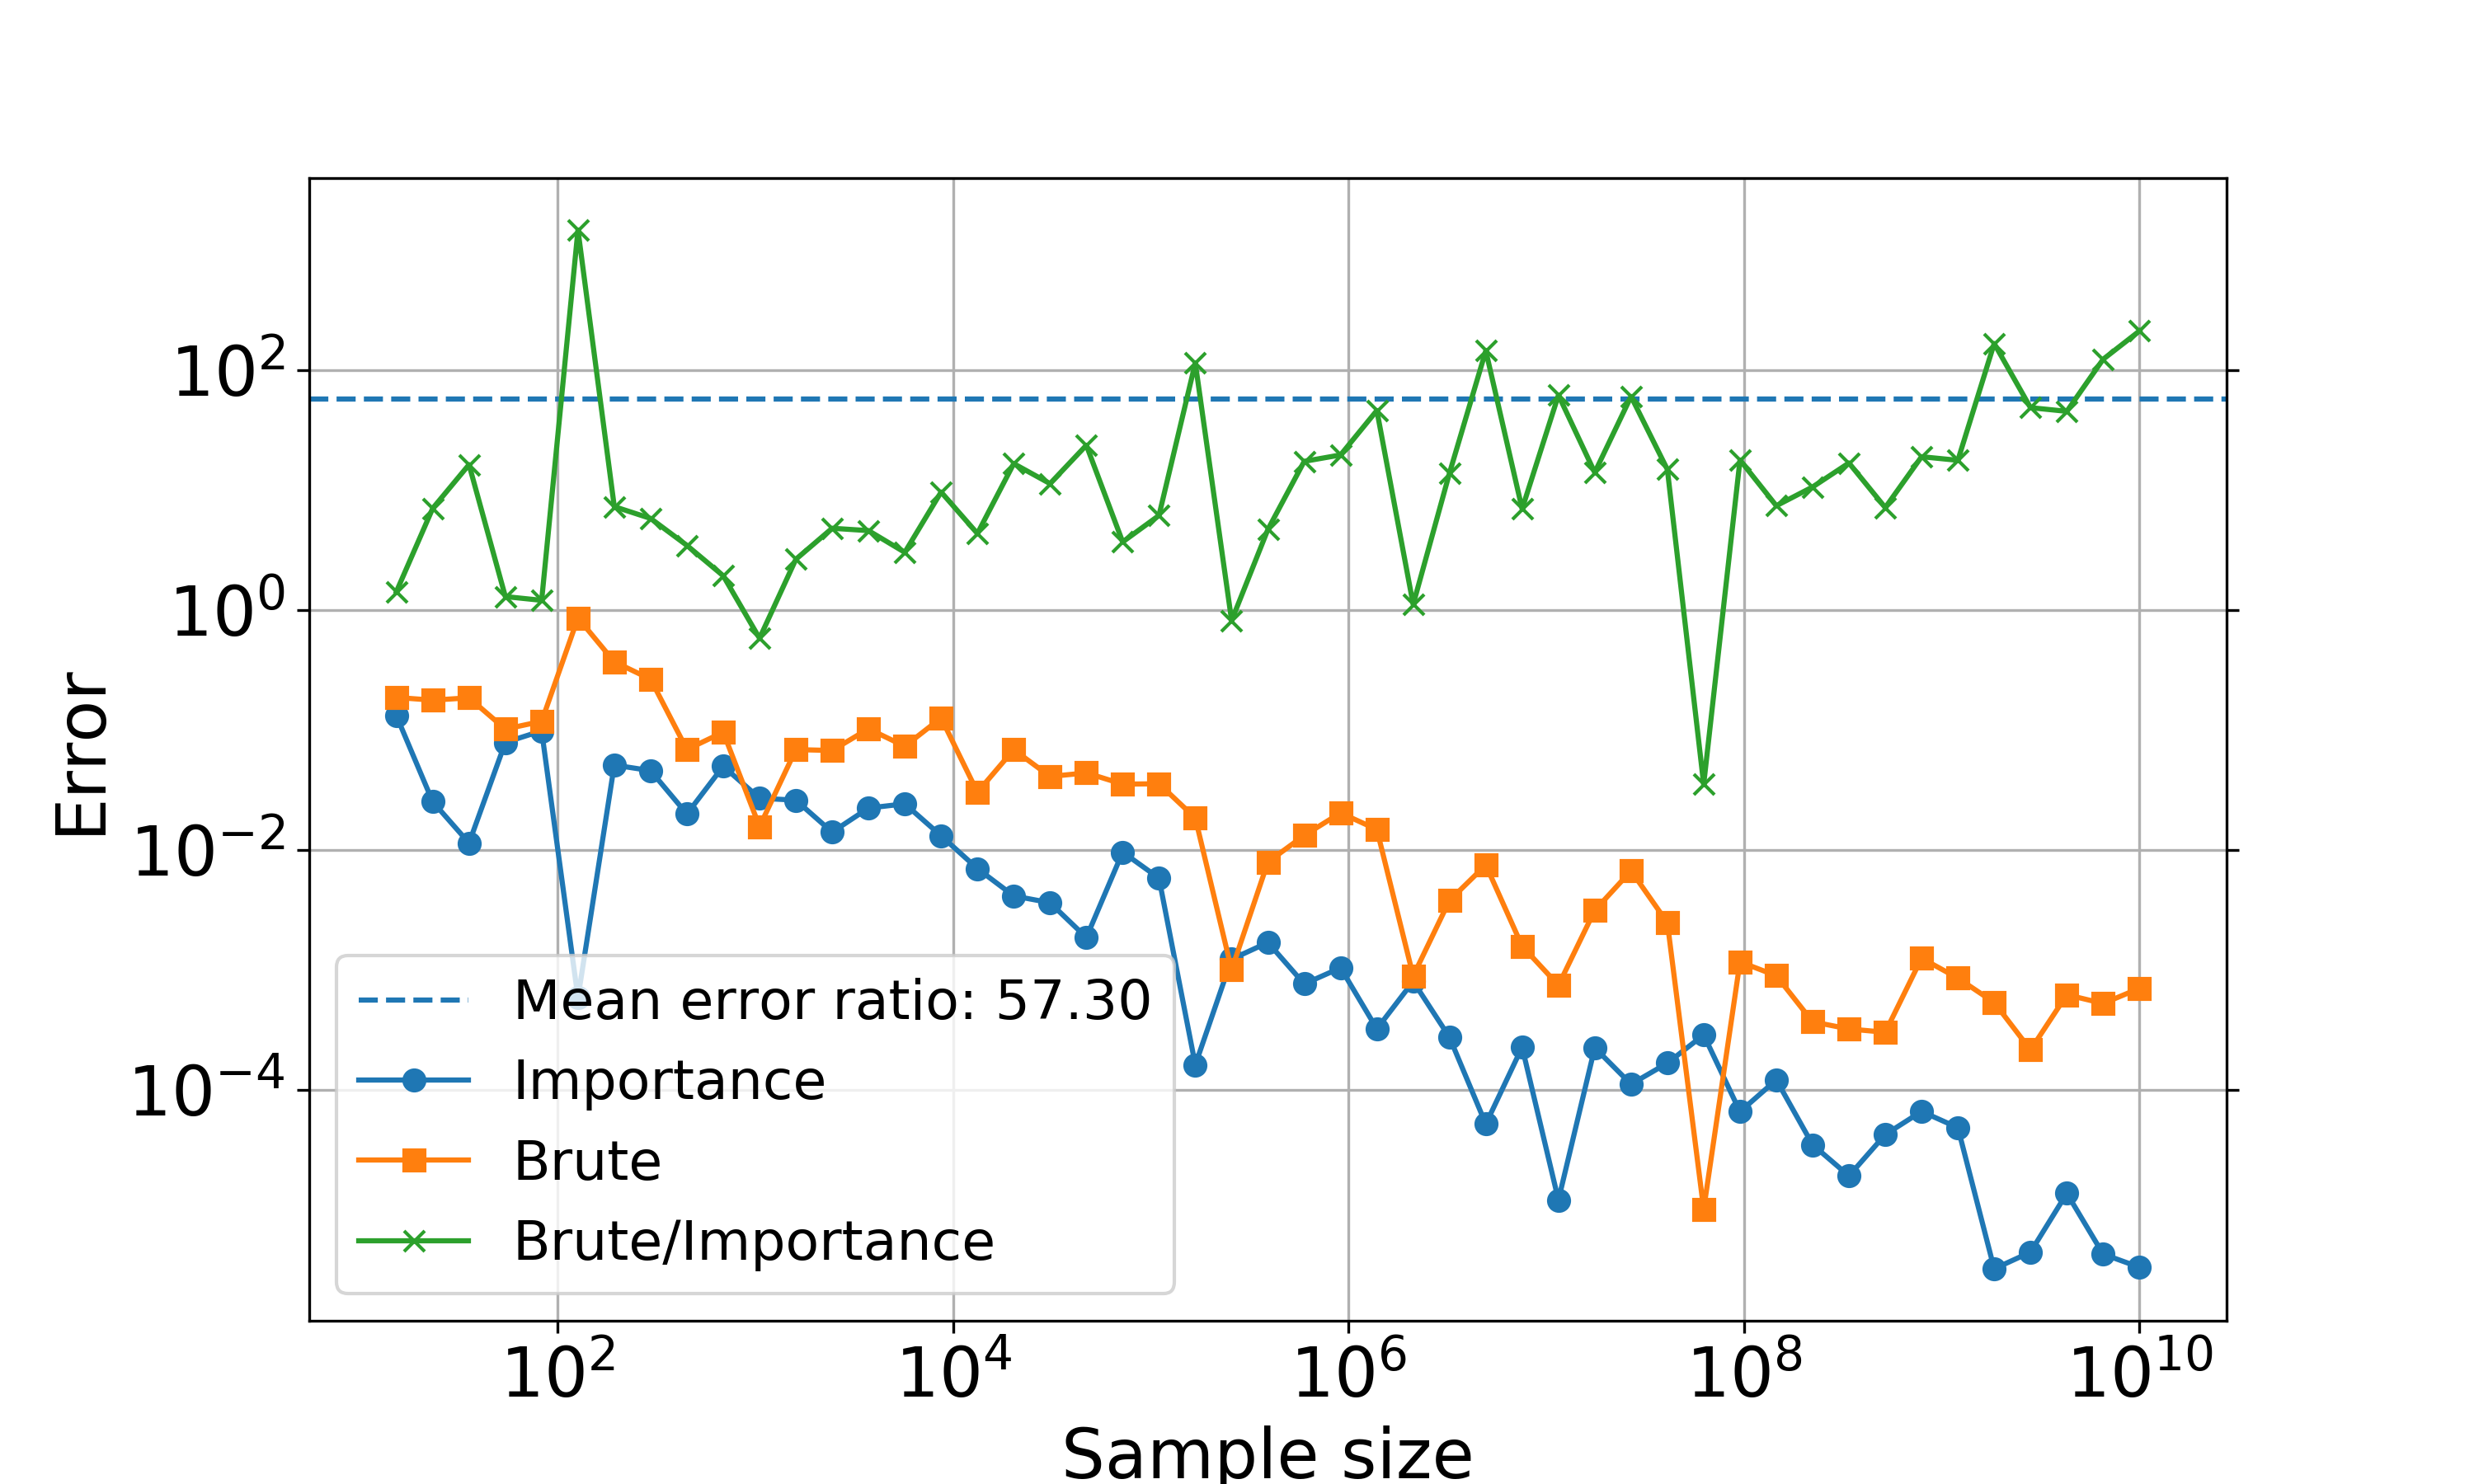
\includegraphics[width=0.8\textwidth]{../figures/mc_error.png}
  \caption{Absolute value of difference between Monte-Carlo results and analytical
  solution using brute force and importance sampling.}

  \label{fig:mc_error}
\end{figure}

To look into the dependence of accuracy on runtime we show \cref{fig:mc_std_time}
which shows standard deviation divided by run time for several N. Taking account
for the run time shows that the importance sampling in this case gets really
effective for $N \geq 10^5$, outperforming the brute force by roughly a factor
40.

\begin{figure}[H]
  \centering
  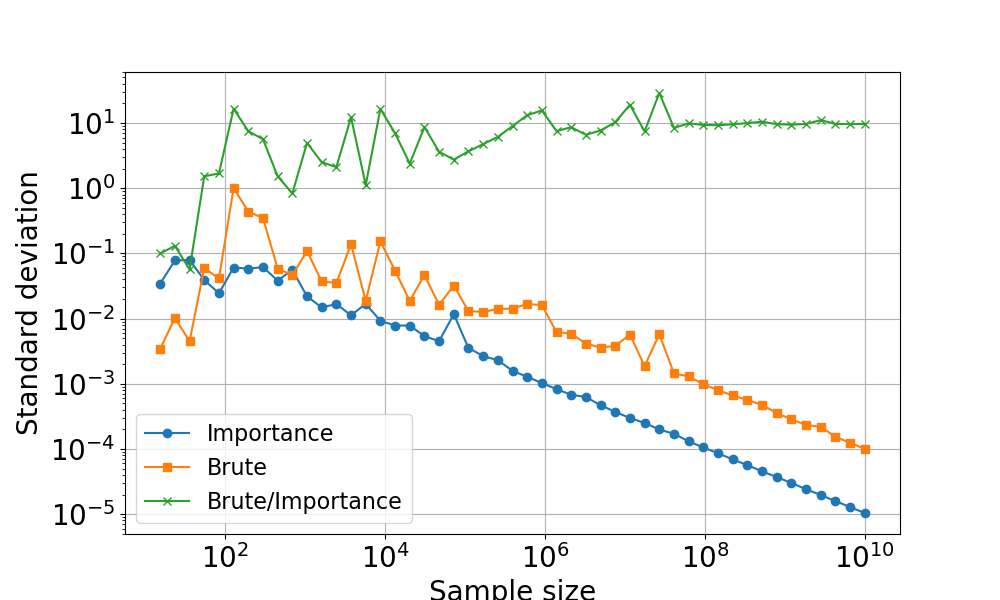
\includegraphics[width=0.8\textwidth]{../figures/mc_std_time.png}
  \caption{Standard deviation divided by run time.}

  \label{fig:mc_std_time}
\end{figure}

\subsubsection{Parallelization}

The results of parallelizing our code is shown in \cref{fig:mc_time_ratio}, which
shows that when N is larger than 10000 we acheived a speedup in the order of 5.
Since the code was run on a laptop with 8 cores this was not optimal, but still
a great boost to the run time.

\begin{figure}[H]
  \centering
  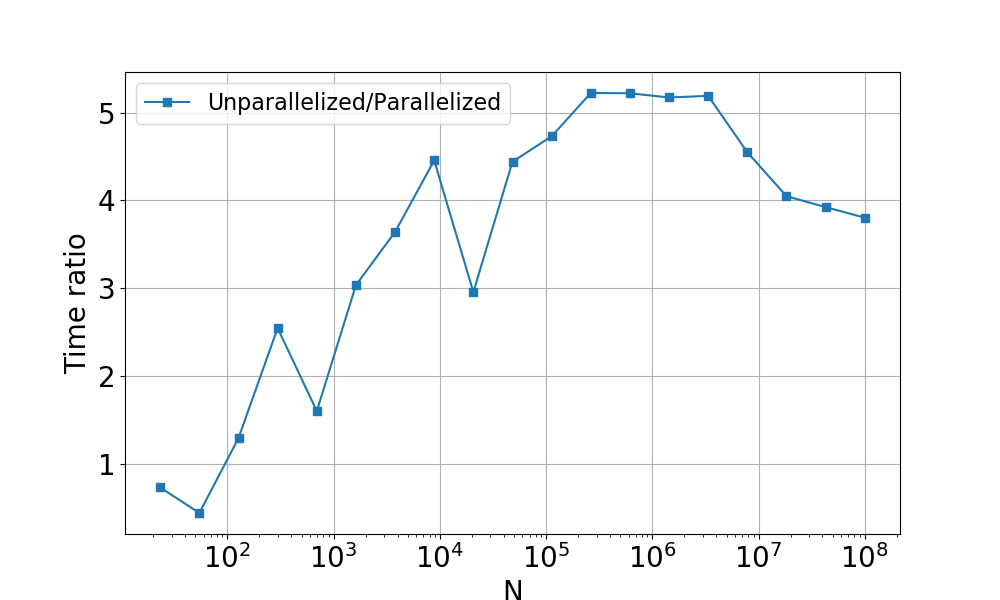
\includegraphics[width=0.8\textwidth]{../figures/mc_time_ratio.png}
  \caption{Run time of unparallelized divided by parallelized version
          of the importance sampling algorithm.}

  \label{fig:mc_time_ratio}
\end{figure}
